\documentclass[a4paper]{article}

\usepackage[utf8]{inputenc}
\usepackage[T1]{fontenc}
%\usepackage[finnish]{babel}
\usepackage[english]{babel}
\usepackage{lmodern}

%\usepackage{graphicx}
\usepackage{enumitem}
\usepackage{amsfonts}
\usepackage{amsmath}
\usepackage{amssymb} %\nmid
\usepackage{amsthm} % \begin{proof}
%\usepackage{bm}
%\usepackage{hyperref}
\usepackage{multicol}
%\usepackage[landscape]{geometry}
\usepackage{tikz}
\usetikzlibrary{arrows,positioning,shapes,fit,calc,arrows.meta,mindmap,trees}
%\usepackage{dtklogos}
%\usepackage{pgfplots}
%\pgfplotsset{compat=1.13}
\usepackage[normalem]{ulem}
\usepackage{float}
\usepackage{mathtools} %, nccmath
%\usepackage{pst-plot, pst-eucl}
\usepackage{tkz-euclide}
%\usetkzobj{all}

\newcommand{\N}{\mathbb N}
\newcommand{\Z}{\mathbb Z}
\newcommand{\R}{\mathbb R}
\newcommand{\C}{\mathbb C}
\newcommand{\Q}{\mathbb Q}

\newcommand{\PS}{\mathcal{P}}
\DeclareMathOperator{\Ima}{Im}

\title{Latex Document
	\\Template}

\author{Anonymous}
\pagestyle{empty}

\begin{document}

\maketitle

%\setlength{\parindent}{0em}
%\setlength{\parskip}{5pt}

\section*{1.}

Bla bla blabla bla simple calculation:

\begin{align*}
(re^{i\delta})^9 &= e^{0i} \\
\implies r^9e^{9i\delta} &= e^{0i}
\end{align*}

The elements $z^i \in \langle z \rangle = \{z^{n\in\N} \mid 0 \leq n \leq 8\}$, \\
spanned by $z = \cos(\frac{2}{9}\pi)+\sin(\frac{2}{9}\pi)i$:

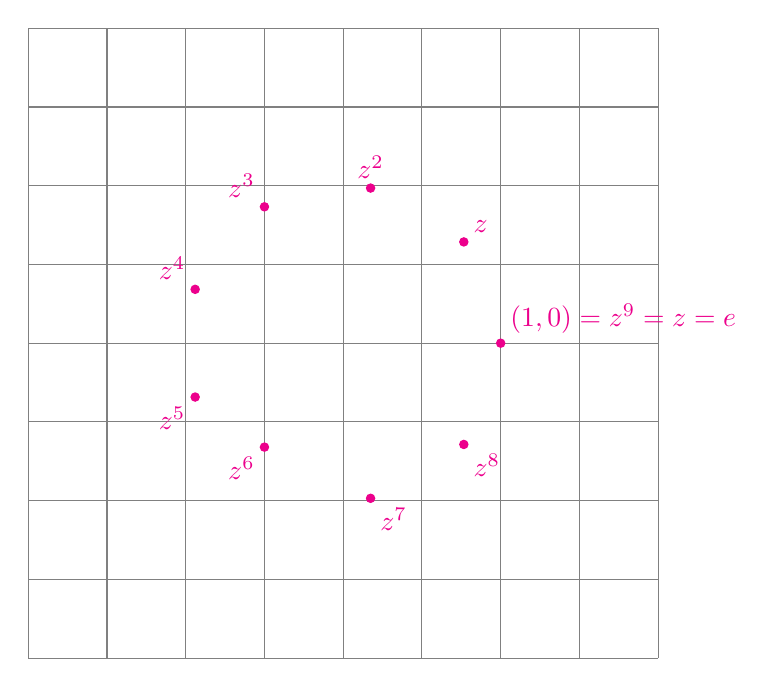
\begin{tikzpicture}[x=2cm,y=2cm]
\tkzInit[xmin=-2,ymin=-2,xmax=2,ymax=2,]
\tkzAxeXY
\tkzGrid
\tkzDefPoints{0.766/0.643/z,
	0.174/0.985/z^2,
	-0.5/0.866/z^3,
	-0.94/0.342/z^4,
	-0.94/-0.342/z^5,
	-0.5/-0.66/z^6,
	0.174/-0.985/z^7,
	0.766/-0.643/z^8,
	1/0/e}
\tkzDrawPoints[size=3,color=magenta](z,z^2,z^3,z^4,z^5,z^6,z^7,z^8,e)
\tkzLabelPoint[above right, color=magenta](z){$z$}
\tkzLabelPoint[above, color=magenta](z^2){$z^2$}
\tkzLabelPoint[above left, color=magenta](z^3){$z^3$}
\tkzLabelPoint[above left, color=magenta](z^4){$z^4$}
\tkzLabelPoint[below left, color=magenta](z^5){$z^5$}
\tkzLabelPoint[below left, color=magenta](z^6){$z^6$}
\tkzLabelPoint[below right, color=magenta](z^7){$z^7$}
\tkzLabelPoint[below right, color=magenta](z^8){$z^8$}
\tkzLabelPoint[above right, color=magenta](e){$(1,0)=z^9=z=e$}
\end{tikzpicture}

More blah blah blaaa

\newpage
\section*{2.}
Some more blah blah

\begin{enumerate}[label=(\alph*)]
	\item Even more text or perhaps the first point or subtask\dots
	\item Second
\end{enumerate}

\end{document}
